\chapter{Progettazione concettuale}
		
		
	\begin{figure}[hbt]
	\section{Class Diagram}
	\centering
	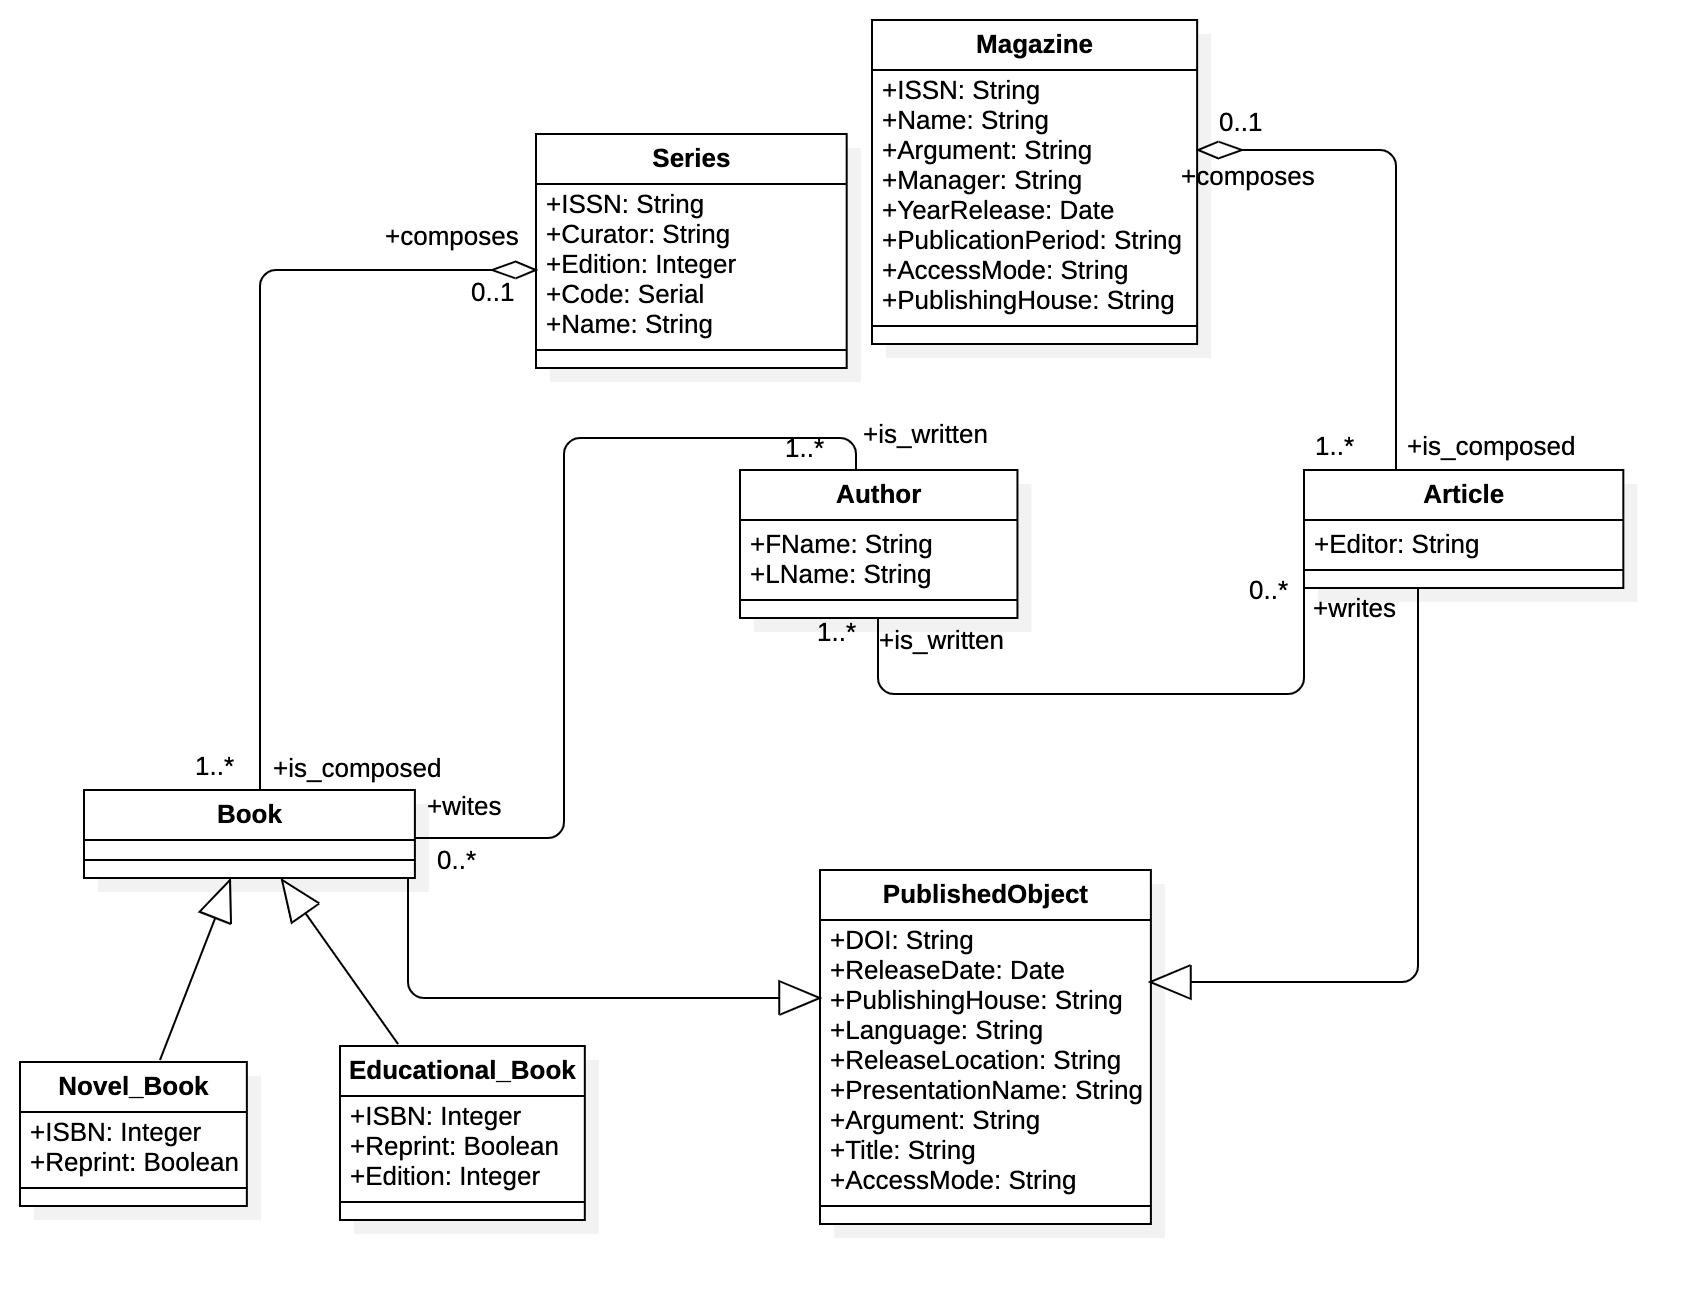
\includegraphics[width=1.1\textwidth]{Immagini/ClassDiagram.png}
	\caption{Class Diagram}
	\label{fig:ClassDiagram}
	\end{figure}

    \section{Analisi della ristrutturazione del Class Diagram}
        
        \subsection{Analisi delle ridondanze}
        
        	Le ridondanze individuate nell class diagram sono presenti nella specializzazione della classe \texttt{Book} in: \texttt{Novel\_Book} e \texttt{Educational\_Book}. \\
        	Gli attributi: \texttt{ISBN} e \texttt{Reprint} di entrambe le specializzazioni vengono inserite all'interno della classe \texttt{Book}.
            
        \subsection{Analisi degli identificativi}
            Identificativo primario per la classe \texttt{Book} è l'attributo \texttt{DOI}, viene attribuito all'attributo \texttt{ISBN} il vincolo di chiave candidata. 
            Per la classe \texttt{Author} viene implementato un attributo aggiuntivo: \texttt{ID\_Author} che sarà chiave primaria.
			Per la classe \texttt{Article} viene usato l'attributo \texttt{DOI} come chiave primaria.
			Per le classi \texttt{Series} e \texttt{Magazine} viene usato come chiave primaria l'attributo \texttt{ISSN}.

        \subsection{Rimozione degli attributi multipli}
            Non sono presenti attributi multipli all'interno del Class Diagram.
        \subsection{Rimozione degli attributi composti}
        	Non sono presenti attributi composti all'interno del Class Diagram.
            
        \subsection{Partizione/Accorpamento delle associazioni}
       		In questo Class Diagram non sono presenti associazioni 1..1 da eliminare.
        \subsection{Rimozione delle gerarchie, delle composizioni}
    	 Nel Class Diagram vengono incorporati nella classe \texttt{Book} le specializzazioni \texttt{Novel\_Book} e \texttt{Educational\_Book} assieme ai rispettivi attributi. All'attributo \texttt{Argument} nel Class Diagram ristrutturato, viene specificato l'argomento educativo (Filosofia, Economia ecc.) oppure all'attributo viene assegnato il valore: Romanzo.\\
        Dato l'interesse di tracciamento delle classi \texttt{Book} e \texttt{Article} in modo separato, viene eliminata la classe \texttt{PublishedObject} e i suoi attributi vengono inseriti all'interno delle classi menzionate precedentemente.
        Le composizioni che riguardano le classi \texttt{Series} e \texttt{Magazine}, vengono eliminate e sostituite da una semplice associazione.
        \newpage
    \section{Class Diagram ristrutturato}
  
    \begin{figure}[hbt]
	\centering
	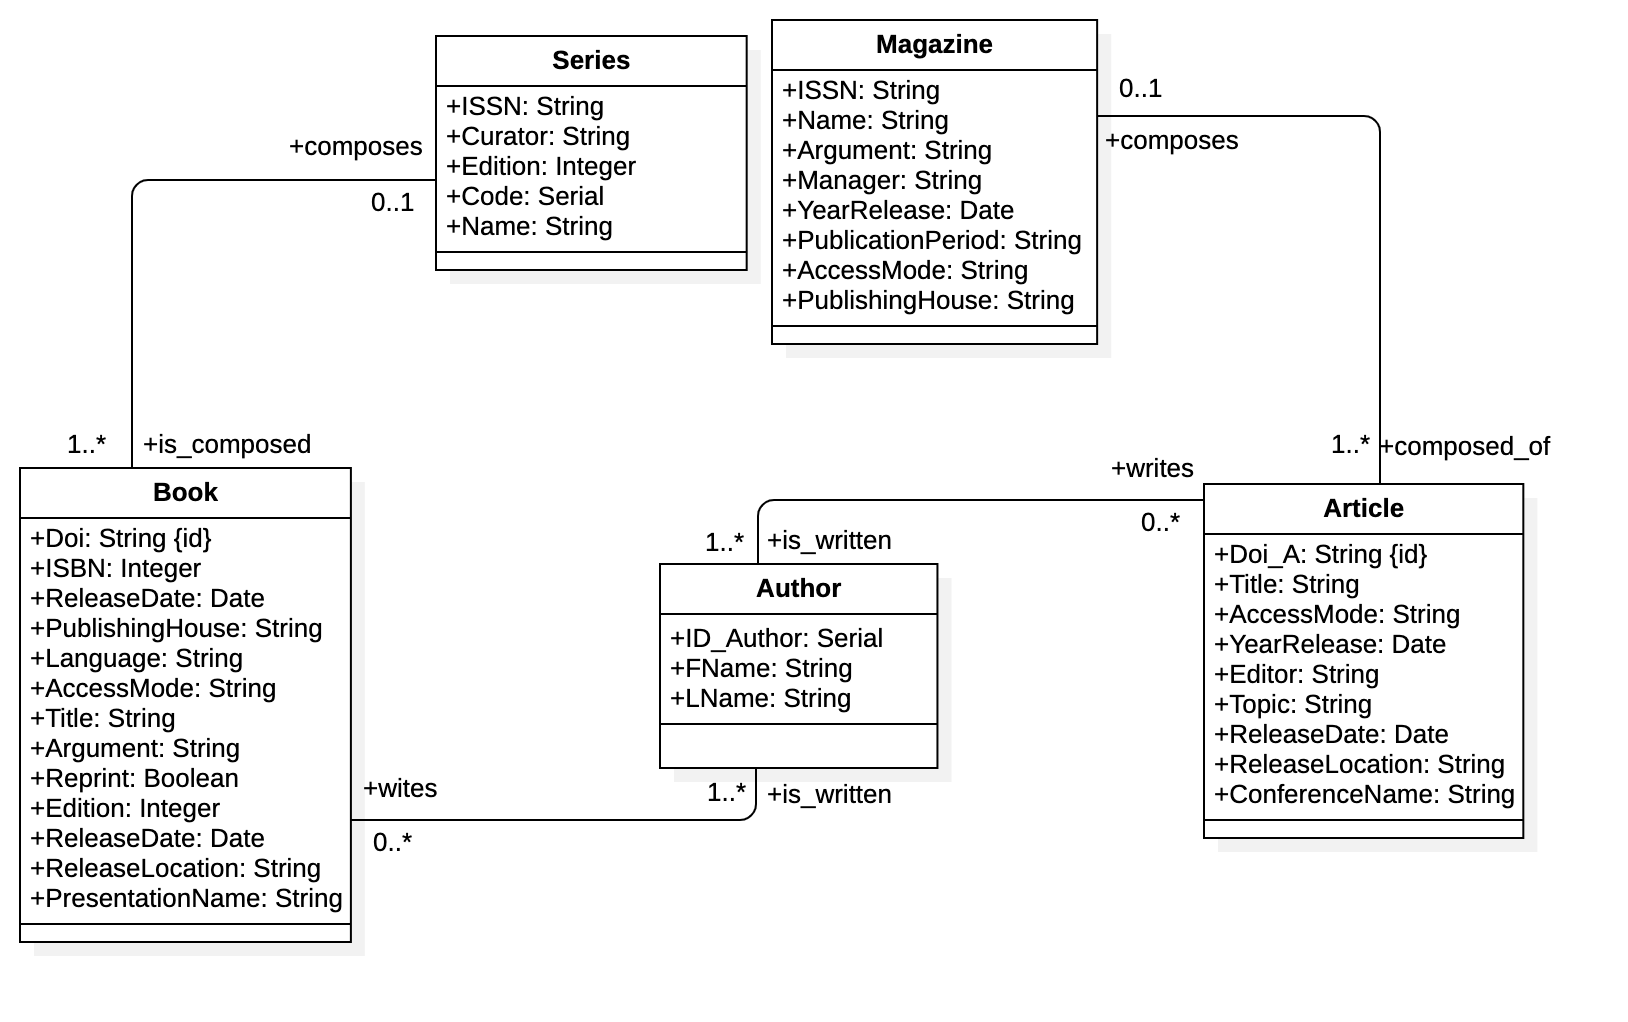
\includegraphics[width=1\textwidth]{Immagini/ClassDiagramRIS.png}
	\caption{Class Diagram \\ Ristrutturato}
	\label{fig:ClassDiagramRIS}
	\end{figure}

\newpage
\begin{table}[]
\section{Dizionario delle classi}
\caption{Dizionario delle Classi}
\label{tab:DizionarioClassi}
\resizebox{\textwidth}{!}{%
\begin{tabular}{|l|l|l|}
\hline
\rowcolor[HTML]{762DC3} 
\textbf{Classe} &
  \textbf{Spiegazione} &
  \textbf{Attributi} \\ \hline
\textbf{Author} &
  Autore di libri o articoli &
  \begin{tabular}[c]{@{}l@{}}ID\_Author (Serial): Author's identification code. \\ FName (String): Author's first  name. \\ LName (String): Author's last name.\end{tabular} \\ \hline
\textbf{Books} &
  \begin{tabular}[c]{@{}l@{}}Oggetti legibili, romanzi o \\ d'educazione\end{tabular} &
  \begin{tabular}[c]{@{}l@{}}DOI(String): Digital object Identifier of the book. \\ ISBN (Integer): Numerical classification sequence of the book. \\ Edition (Integer): Edition number. \\ AccessMode (AccessMode): Fruition method. \\ ReleaseDate (Date): Publication date. \\ PublishingHouse (String): Publishing house that printed the book. \\ ReleaseLocation (String): Place of  publication of the book. \\ Language (String): Language in which the book is written. Title (String): Book title. \\ Argument (String): Book topic. \\ Reprint (Boolean): Parameter that identifies if the book is a reprint or not. \\ PresentationName (String): Name of  pesentation in which books are presented.\end{tabular} \\ \hline
\textbf{Series} &
  Insieme di libri &
  \begin{tabular}[c]{@{}l@{}}ISSN (String):International number that identifies serial publications.\\ Edition (Integer):Edition number. \\ Curator (String):Curator of the series. \\ Code (Serial):Code assigned to the series. \\ Name (String): Series' name.\end{tabular} \\ \hline
\textbf{Magazine} &
  Insieme di Articoli &
  \begin{tabular}[c]{@{}l@{}}(Integer): International number that identifies serial publications. \\ Name (String): Magazine's name. \\ Argument (String): Magazine topic. \\ Manager (String): Event organizer. \\ YearRelease (Date): Publication year. \\ PublicationPeriod (String): Periodicity of publication. \\ AccessMode (AccessMode): Fruition method.\end{tabular} \\ \hline
\textbf{Article} &
  Articoli di ricerca Scientifica &
  \begin{tabular}[c]{@{}l@{}}DOI (String): Digital object Identifier of the book.\\ Title (String): Book title.\\ AccessMode (AccessMode): Fruition method. \\ YearRelease (Date):Publication year. \\ Editor (String):Article editor. \\ ReleaseDate (Date):Publication date.\\ ReleaseLocation (String):Place of publication of the book.\\ ConferenceName (String): Name of pesentation in which books are presented.\end{tabular} \\ \hline
\end{tabular}%
}
\end{table}

\newpage


\begin{table}
\section{Dizionario delle associazioni}
\centering
\caption{Tabella delle Associazioni}
\resizebox{\linewidth}{!}{%
\begin{tabular}{|l|l|l|}	
\hline
\rowcolor[HTML]{762DC3} \multicolumn{1}{|r|}{Nome} & Descrizione                                                                                                                            & Classi Coinvolte  \\
composes/is\_composed                                        & \begin{tabular}[c]{@{}l@{}}Una collana è composta da uno o più libri/\\ Un libro può comporre oppure no una collana\end{tabular}       & Series/Book       \\ 
\hline
writes/is\_written                                           & \begin{tabular}[c]{@{}l@{}}Un libro è scritto da uno o più autori/\\ Un autore scrive molti oppure nessun libro\end{tabular}           & Book/Author       \\ 
\hline
is\_written/writes                                           & \begin{tabular}[c]{@{}l@{}}Un autore scrive molti oppure nessun articolo/\\ Un articolo è scritto da uno o più autori\end{tabular}     & Author/Article    \\ 
\hline
composes/is\_composed                                        & \begin{tabular}[c]{@{}l@{}}Un articolo puo comporre oppure no una rivista/\\ Una rivista è composta da uno o più articoli\end{tabular} & Article/Magazine  \\
\hline
\end{tabular}
}
\end{table}